\subsection{Müze Turu}
\indent\indent Türk İslam Müzesi, adından da anlaşılacağı gibi ağırlıklı olarak Türk ve İslam eserlerinin sergilendiği bir müze. Müze, 2012-2014 yılları arasında geçirdiği restorasyondan sonra günümüzdeki halini almıştır. Müzedeki eseler, ait oldukları dönemlere göre tasnif edilmiş olarak ayrı odalarda sergilenmektedir. Sırasıyla Abbasiler, Emeviler, Büyük Selçuklular, İlhanlılar, Timurlular, Memlûkler, Safeviler, Kaçarlar, Anadolu Selçuklular ve Osmanlılar dönemlerinden kalan eserler bulunmaktadır. Müzede öne çıkan eserler arasında el yazmaları, halı ve kilimler, Kutsal Emanetler ve şamdanlar ön plana çıkmatadır.
\subsubsection{Lahitler ve Kitabeler}
\indent\indent Müzenin girişinde iki mermer lahit bulunmakta(Şekil \ref{fig:lahit}). Bu lahitler Memlûk Halep Valisi Özdemir ve eşinini mezarları için tasalanmış olup, 1493 yılına aittir. Lahitler, ya mezarın üstüne ya da yakınına konuşlandırılan ve mezar taşı görevi taşıyan yapılardır. Yaygın kanının aksine içinde naaşı muhafaza etmemektedir.\newline
\indent Bu kısmı geçip, soldaki kapıdan devam edince karşımıza iki tane kitabe çıkıyor. Şekil \ref{fig:grave}'deki kitabe , Emeviler döneminden bir mescide aittir. Şekil \ref{fig:road_stone}'deki kitabe  ise bir mesafe taşıdır. Bu kitabe, günümüzde kilometre tabelalarının Emeviler dönemindeki eşleniğidir. Mesefa taşı kitabesi, en geç 705 yılına aittir.\newline
\begin{figure}[ht]
    \centering
    \subfigure[Özdemir ve Eşinin Lahitleri]{
        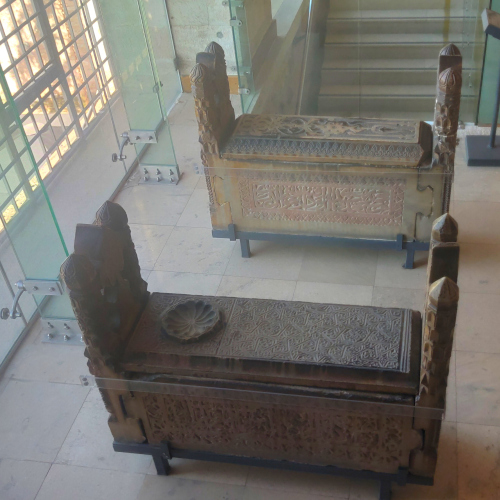
\includegraphics[height=0.3\textheight,width=0.30\linewidth]{assets/lahit.jpg}
        \label{fig:lahit}
    }
    \hfill
    \subfigure[Mescit Kitabesi]{
        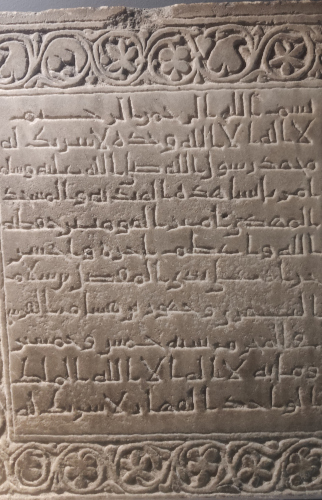
\includegraphics[height=0.3\textheight,width=0.30\linewidth]{assets/mescid.jpg}
        \label{fig:grave}
    }
    \hfill
    \subfigure[Mesafe Taşı Kitabesi]{
        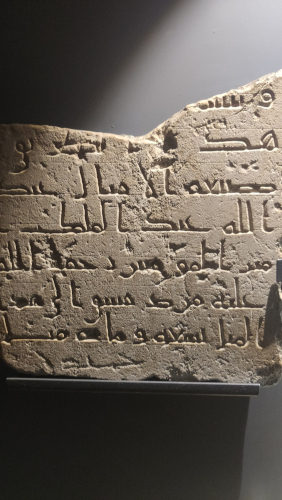
\includegraphics[height=0.3\textheight,width=0.30\linewidth]{assets/mesafe.jpg}
        \label{fig:road_stone}
    }
    \caption{Lahitler ve Kitabeler}
    \label{fig:lahits_kitabes}
\end{figure}
\subsubsection{Samarra Camii ve Rakka Seramikleri}
\begin{wrapfigure}{r}{0.4\textwidth}
    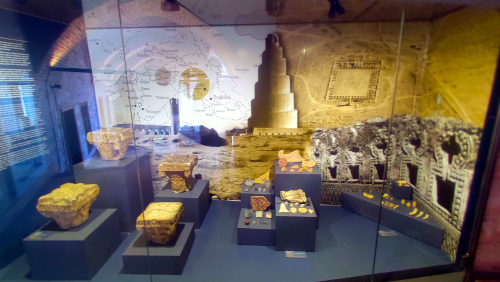
\includegraphics[width=0.4\textwidth]{assets/samarra.jpg}
    \caption{Samarra Camii}
    \label{fig:samarra}
    \vspace{10pt}
    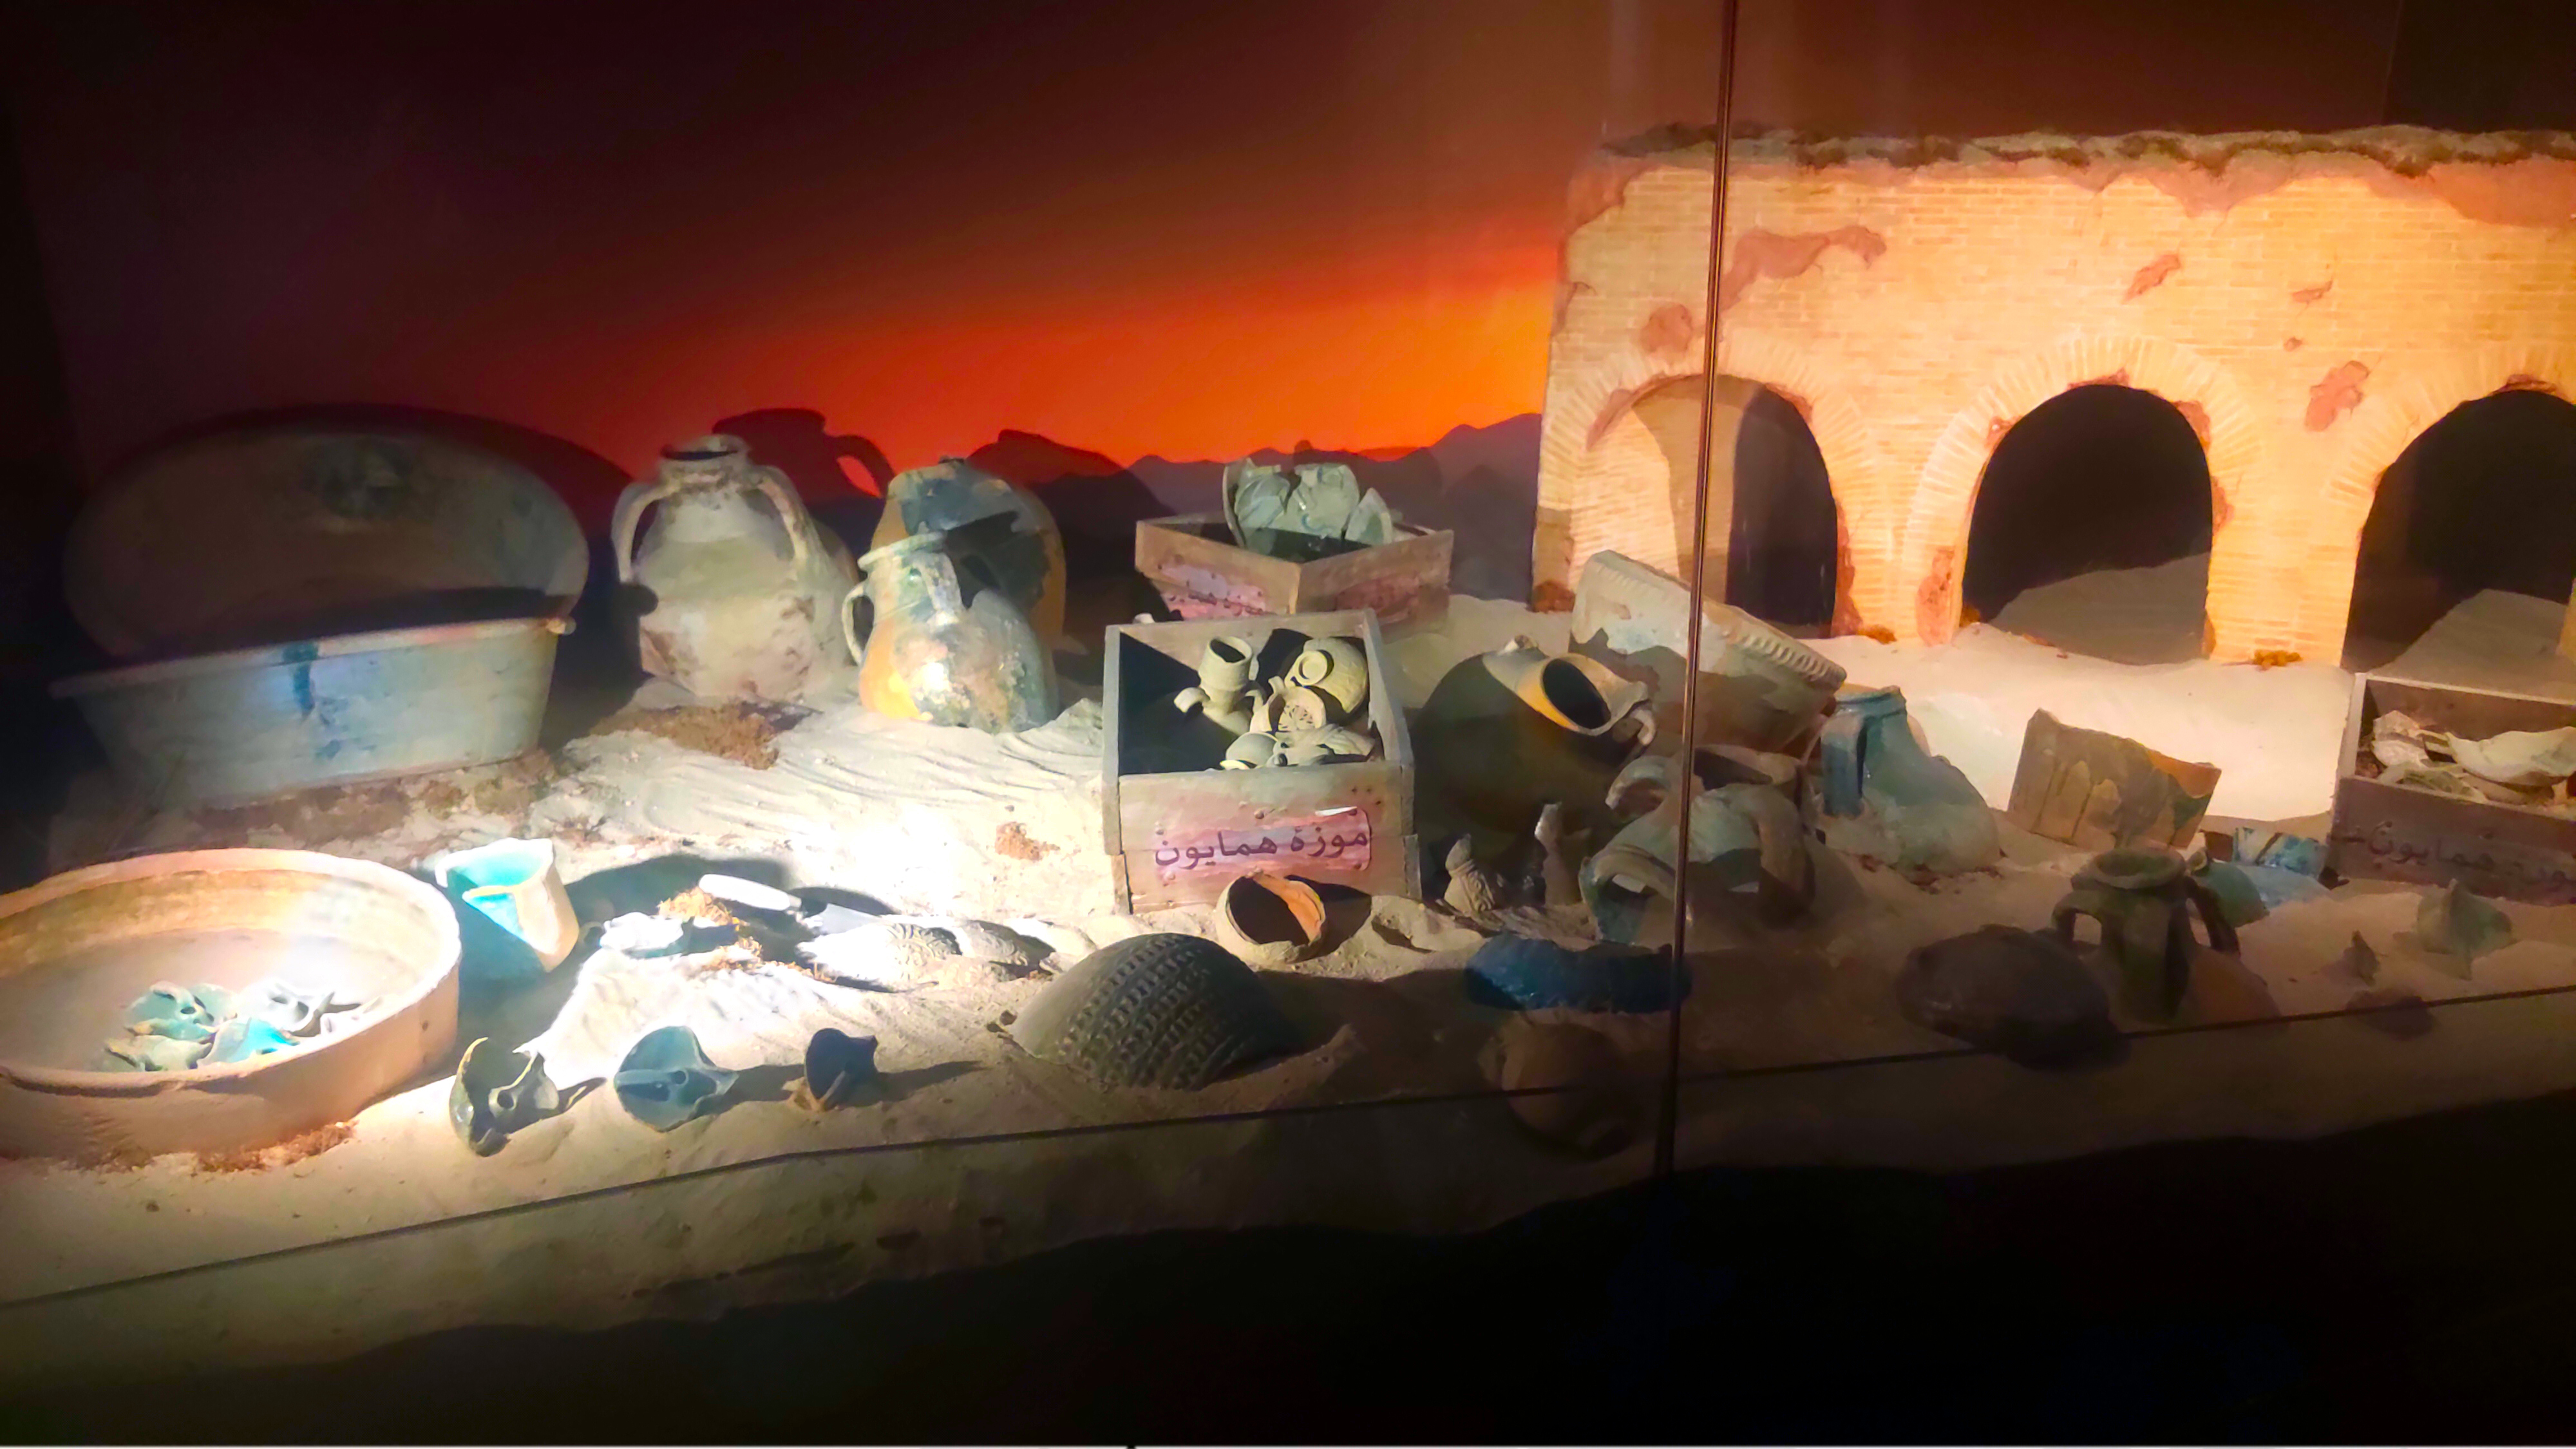
\includegraphics[width=0.4\textwidth]{assets/raqqa.jpg}
    \caption{Rakka Seramikleri}
    \label{fig:raqqa}
\end{wrapfigure}
\indent Lahitler ile kitabeler arasındaki bölümde, Samarra Camii'nin kalıntılarını ve planını gösteren sergi karşımıza çıkıyor. Dönemin Abbasi halifesi el-Mu'tasım'ın ordusu, ağırlıklı olarak Türk askerlerini içerirdi. Bu askerleri başkent Bağdat'ta barındırılması, bir süre sonra hem şehrin güvenliği hem de halkın huzuru üzerinde sorun teşkil etmeye başladı. Bundan dolayı halife el-Mu'tasım, Türk birlikleri yerleştirmek ve askeri üs oluşturmak için, Bağdat'ın 125 kilometre kuzeyine 836 yılında Samarra şehrini kurdu. 848 yılında Abbasi halifesi Mütevekkil tarafından yapımına başlanan Samarra Camii, 852 yılında tamamlanmıştır. 1250 civarında, Moğol akınları sırasında yerle bir edilen camiinin günümüze sadece minaresi ulaşmıştır. İslâm mimarisinde nadir rastlanan bir tarza sahip olan ve Babil zigguratlarını andıran minare, spiral şekilde yükselmektedir. Şehrin bir askeri üs olduğu düşünüldüğünde, minarenin bir istihkâm olarak kullanılması düşünülmüş olabilir.\newline
\indent Kitabelerin bulunduğu odadaki sergide ise Rakka seramikleri bulunmaktadır. Eyyübiler döneminde bölge ekonomisinin temel direğini seramikçilik oluşturmaktaydı. 19. yüzyıl sonlarında yapılan kazılar ile ortaya çıkan Rakka seramik eserleri burada sergilenmektedir. Şekil \ref{fig:raqqa}'de görülen sandıklar üzerinde \textit{Müze-i Hümayûn} yazmaktadır. Eserlerin Türk İslâm Müzesi'nden önceki durağı İstanbul Arkeoloji Müzesi olmalıdır.\newline 
\subsubsection{El Yazması Eserler}
\indent\indent Müzede, 2500 civarında yazma eser bulunmaktadır. El yazmaları, ağırlıklı olarak Kur'an-ı Kerim, cüz ve mecmua tarzı eserleri ihtiva etmektedir.\newline
\indent Müzede Emevi, Memlûk, İlhanlı, Timur, Safevi ve Kaçar dönemlerine ait el yazması Kur'an-ı Kerim ve cüz eserler dönemlerine göre ayrı odalarda tasnif edilmiş halde sergilenmektedir. Bu eserlerden Emevi dönemi el yazması Kur'an-ı Kerim büyüklüğü ile ilgi çekicidir. İlhanlı dönemine ait Kur'an-ı Kerim'de ise tefsir çalışması mevcuttur. Tefsir, satırların altına kırmızı kalem ile işlenmiştir. Memlûk ve Safevi el yazmalarında tezhip(Arapça \textit{zeheb(altın)} kelimesinden altınlamak anlamında) sanatının nadide işçiliği gözlemlenebilir. Şam Emevi Camii'nden 1917 yılında getirilerek, Şam Evrakı koleksiyonu şeklinde sergilenen eserler arasında parşömen üzerine Kur'an sayfaları 846 gibi erken bir tarihe uzanmakta ve İslâm sanatının ilk örneklerini ouşturmaktır. Şam Evrakı Koleksiyonunda Kur'ân yapraklarının yanı sıra, 8. yüzyıl sonundan 19. yüzyıla kadar uzanan bir periyodda yazılmış ciltler ve belgelere de bulunmaktadır.\newline
\indent Kur'an-ı Kerim ve cüz eserlerin yanı sıra az sayıda mecmua eserler de el yazması eserler arasında bulunmaktadır. Bu eserler arasinda Timur döneminden Hamse-i Attar(beş mesneviden oluşan külliyat) ve Memlûk döneminden Kitab-ı Buzuğ El Hilal adında bir mecmua dikkat çekmektedir.
\begin{figure}[H]
    \centering
    \subfigure[Hamse-i Attar]{
        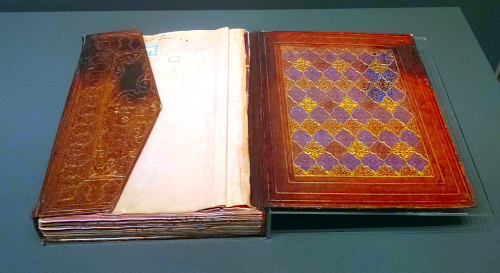
\includegraphics[height=0.2\textheight, width=0.45\linewidth]{assets/hamsei_attar.jpg}
    }
    \hfill
    \subfigure[Kitab-ı Buzuğ El Hilal]{
        \includegraphics[height=0.2\textheight, width=0.45\linewidth]{assets/kitabi_buzug_el_hilal.jpg}
    }
    \caption{El Yazması Mecmua Eserler}
\end{figure}
\begin{figure}[H]
    \centering
    \subfigure[İlhanlı Dönemi Kur'an Kerim ve Tefsir Çalışması]{
        \includegraphics[width=0.9\linewidth]{assets/ilhanli_kuran_tefsir.jpg}
        \label{fig:ilhanli_tefsir}
    }
    \vspace{10pt}
    \subfigure[Emevi Dönemi Kur'an-ı Kerim]{
        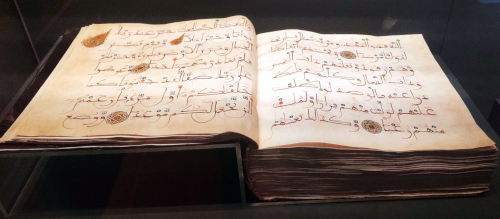
\includegraphics[height=0.2\textheight, width=0.45\linewidth]{assets/emevi_kuran.jpg}
        \label{fig:emevi}
    }
    \hfill
    \subfigure[Memlûk Dönemi Kur'an-ı Kerim]{
        \includegraphics[height=0.2\textheight, width=0.45\linewidth]{assets/memluk_kuran.jpg}
        \label{fig:memluk_kuran}
    }
    \vspace{10pt}
    \subfigure[Safevi Dönemi Kur'an-ı Kerim]{
        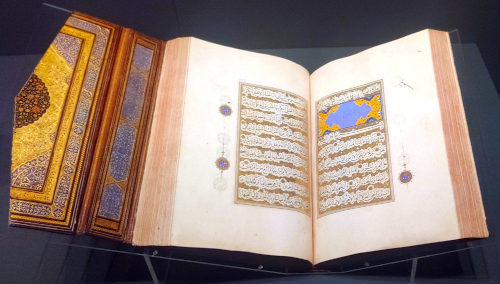
\includegraphics[height=0.2\textheight, width=0.45\linewidth]{assets/safevi_kuran.jpg}
        \label{fig:safevi_kuran}
    }
    \subfigure[Kaçar Dönemi Kur'an-ı Kerim]{
        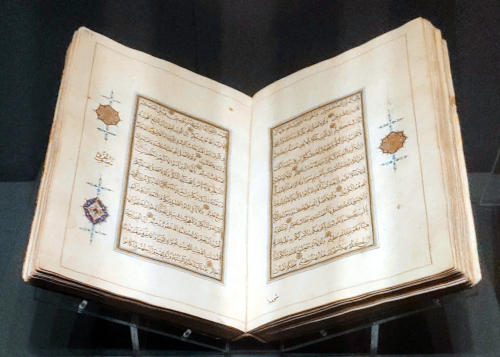
\includegraphics[height=0.2\textheight, width=0.45\linewidth]{assets/kacar_kuran_mesnevi.jpg}
        \label{fig:kacar_kuran_mesnevi}
    }
    \caption{El Yazması Kur'an-ı Kerim ve Cüz Eserler}
    \label{fig:quran}
\end{figure}
\subsubsection{Kutsal Emanetler}
\begin{wrapfigure}{r}{0.25\textwidth}
    \centering
    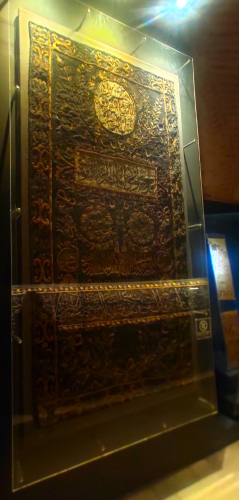
\includegraphics[width=0.20\textwidth]{assets/kabe.jpg}
    \caption{Kabe Örtüsü}
    \label{fig:kabe}
\end{wrapfigure}
\indent\indent Müzede, kutsal emanetler için ayrı bir bölüm oluşturulmuş. Burada dikkat çeken eserlerin başında Kâbe örtüsü bulunmaktadır. Hz. Ömer zamanında başlayan bir gelenek olarak Kâbe örtüsü masrafları devlet hazinesinden karşılanıyordu. Memlûk sultanları döneminde bu örtünün dokunması Mısır'da yapılmaya başlandı. 1517 yılında Yavuz Sultan Selim Mısır'ı fethendice, eski usûle bağlı kalarak örtünün Mısır'da dokunmasını buyurdu. Kanuni Sultan Süleyman zamanında dış örtünün Mısır'da, iç örtünün ise İstanbul'da dokunması kararlaştırıldı. III. Ahmed döneminden itibaren hem iç, hem de dış örtü İstanbul'da dokunmaya başlandı. Sultan Abdülaziz'in 1861'de tahta çıkması münasebetiyle gönderilen örtü, 1943 yılına kadar kullanıldı. I. Dünya Savaşı sırasında bölgenin Osmanlı Devleti'ne karşı ayaklanması ile örtülerin dokuması Mısır'da yapılmaya başlanmıştır. 1962 yılından itibaren örtülerin dokuması Mekke'de kurulmuş fabrikada yapılmaktadır.\cite{dia_4}\newline
\indent Bu kısımdaki bir diğer ilgi çekici eser ise hac vekaletnameleridir. Günümüzde de uygulanmaya devam eden vekalet ile hac uygulaması, geçmişte daha sık başvurulan yöntemdi. Hac yapmakla mükellef kişi bir sağlık sorunu, yaşlılık gibi sebeplerden dolayı başka bir kişiyi vekil olarak gönderebilmektedir. İşte bu vekilliği belgeyen vekaletnamelerin nüshaları burada incelenebilmektedir.\newline
\indent İç kısımda ise el yazmaları bulunmaktadır. Burada el yazması Kur'ân-ı Kerimlerden bir tanesinin Hz. Osman döneminde, bir diğerinin ise Hz. Ali döneminde yazıldığı rivayet edilmektedir. Yine Aşere-i Mübeşşere'nin(Hz. Muhammed tarafından cennetle müjdelenen on kişi) isimlerinin yazılı olduğu örtü de bu alanda sergilenmektedir. Bunların dışında eski bir Kâbe kapısı kilidi ve Kâbe mührü gibi eserler de burada görülebilir.
\begin{figure}[H]
    \centering
    \subfigure[Hz. Osman Dönemi Kur'ân-ı Kerim]{
        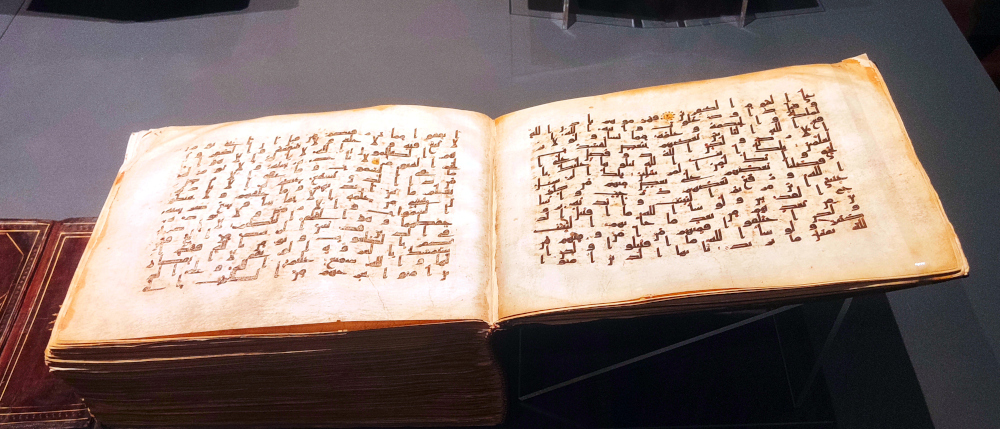
\includegraphics[height=0.2\textheight, width=0.45\linewidth]{assets/osman.jpg}
    }
    \hfill
    \subfigure[Hz. Ali Dönemi Kur'ân-ı Kerim]{
        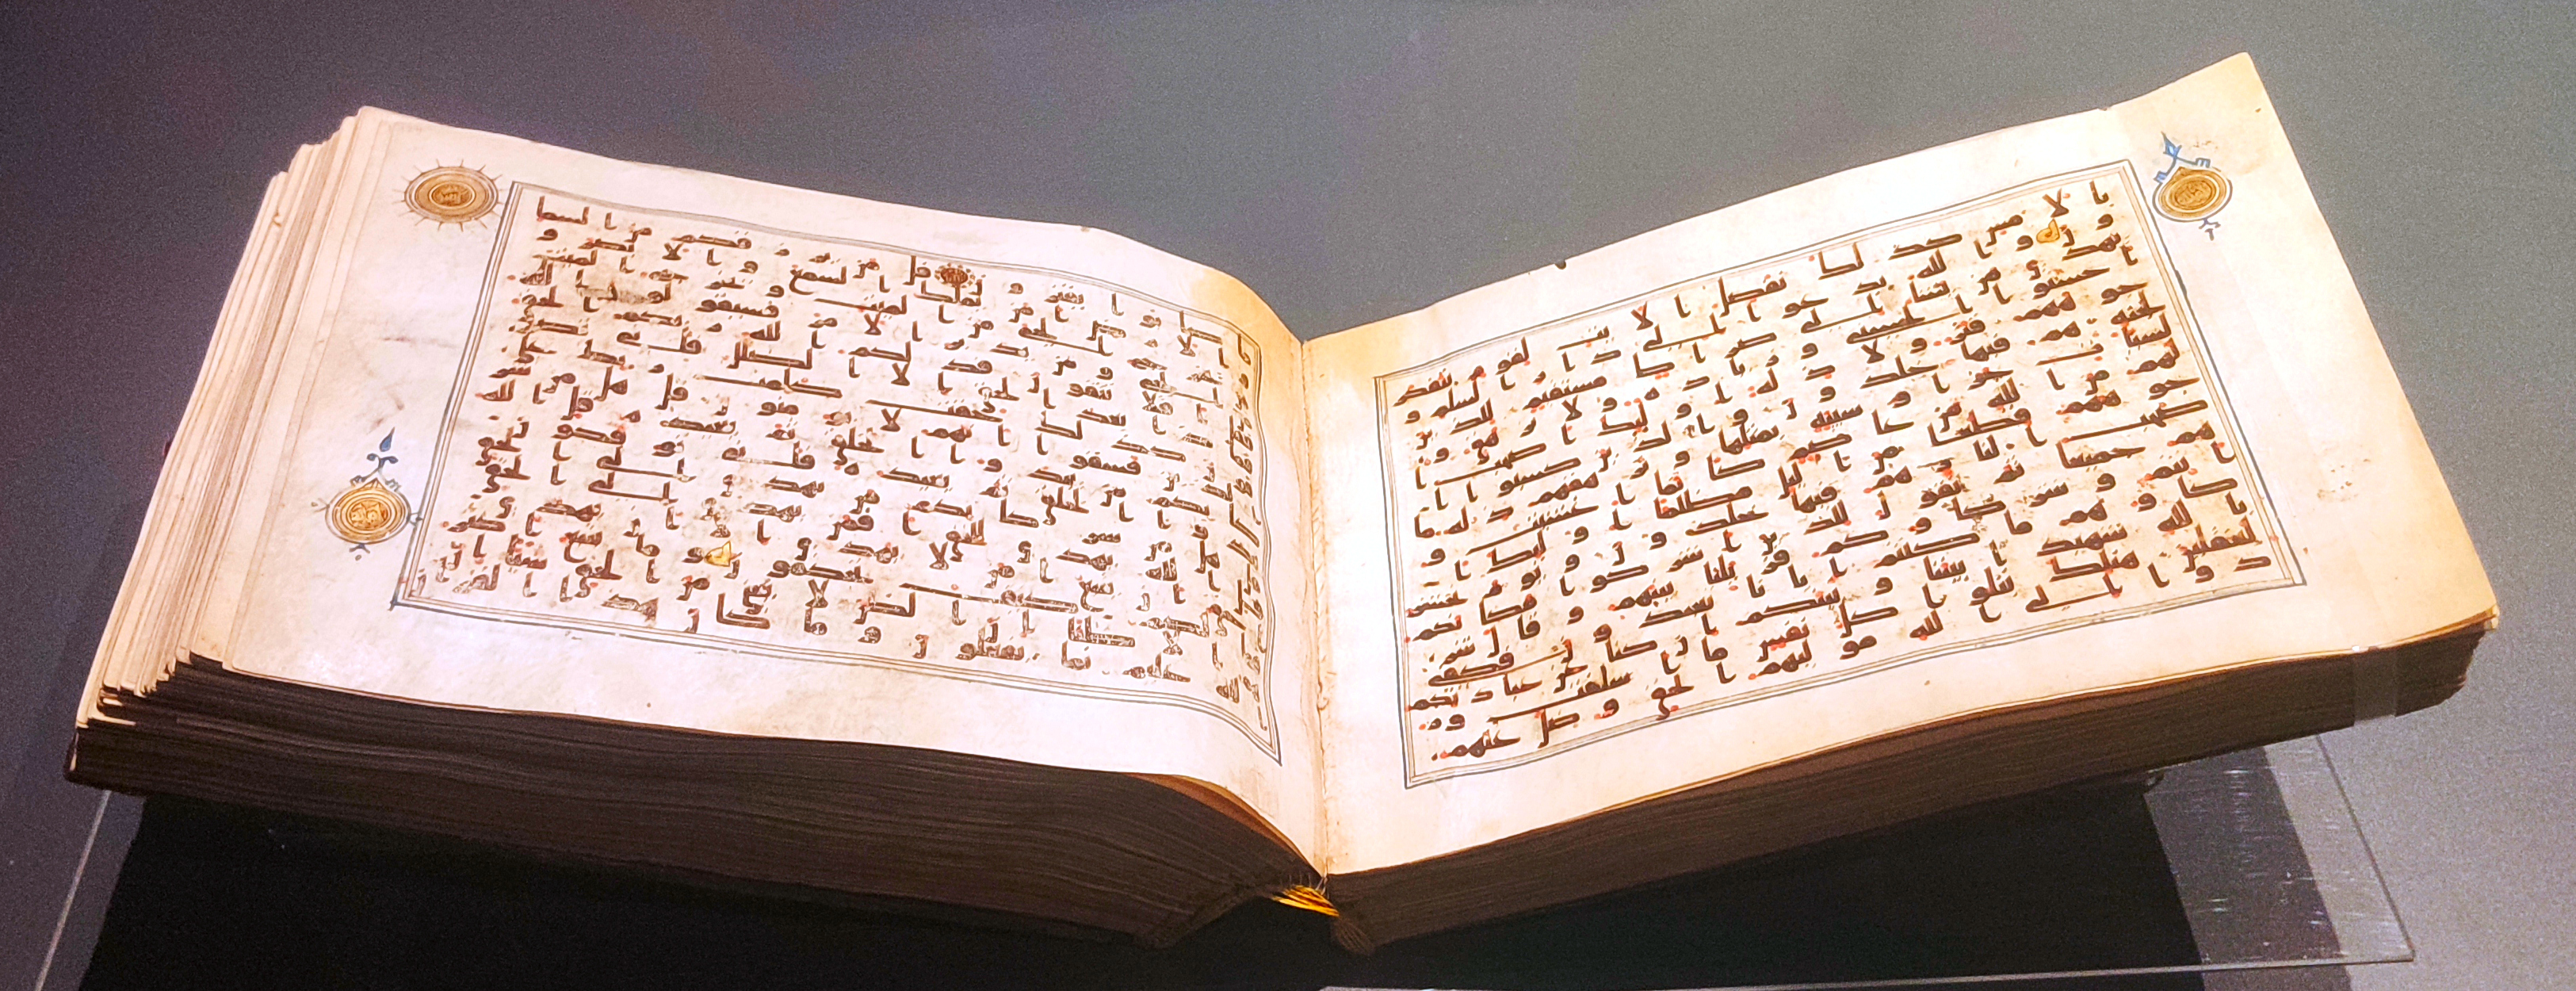
\includegraphics[height=0.2\textheight, width=0.45\linewidth]{assets/ali.jpg}
    }
    \caption{Halife Dönemi El Yazması Kur'ân-ı Kerimler}
\end{figure}
\subsubsection{Diğer Eserler}
\begin{wrapfigure}{r}{0.3\textwidth}
    \centering
    \includegraphics[width=0.3\textwidth]{assets/cizre.jpg}
    \caption{Ulucamii Kapısı}
\end{wrapfigure}
\indent\indent Müzede dikkat çeken bir başka eser ise Cizre Ulucamii kapısıdır. Cizre Ulucamii, Abbasiler döneminde kiliseden camiiye çevrilmiş ve tamir edilmiştir. Artuklular döneminde(1160) yeniden inşa ettirilmiştir. Kapıları 1946 yılında onarılmış ve yapı 2007 yılında Vakıflar Genel Müdürlüğü tarafından restore edilmiştir. Cizre Ulucamii'nin en dikkat çekici unsuru bronzdan yapılmış kapısı ve tokmaklarıdır. Tokmaklar, iki ejderin arasında bir aslan başı şeklinde tasarlanmıştır. Tokmaklardan biri, 1969 yılında yurt dışına kaçırılmıştır.\cite{dia_5}\newline
\indent Müzede, çeşitli dönemlere ait şamdanlar, buhurdanlıklar, yağdanlıklar, seramik eşyalar, keşküller(yarımküre biçiminde bir tür tas), erken dönem astronomik aletler de bulunmakta. Büyük Selçuklular dönemine ait tabure, matara ve reçellikler, yıllar geçse de insanların ihtiyaçlarının aşağı yukarı aynı kaldığını gösteriyor bizlere. Yine aynı galeride bulunan Selçuklu seramik yıldızının örnekleri, Konya Karatay Medresesi Müzesi'nde de bolca bulunmaktadır. Bir diğer ilginç eser ise Kaçar döneminden kalma lakeden yapılmış oyun kartları ve kalemliklerdir. Oyun kartları, Antik Mısır'da oynanan \textit{Senet} oyununun bir benzeri gibi durmaktadır. Fakat aradaki yaklaşık 5000 yıllık zaman farkını düşününce, bu ihtimal çok ufaktır.
\newpage
\clearpage
\begin{figure}[!ht]
    \centering
    \subfigure[Selçuklu Dönemi Seramikleri]{
        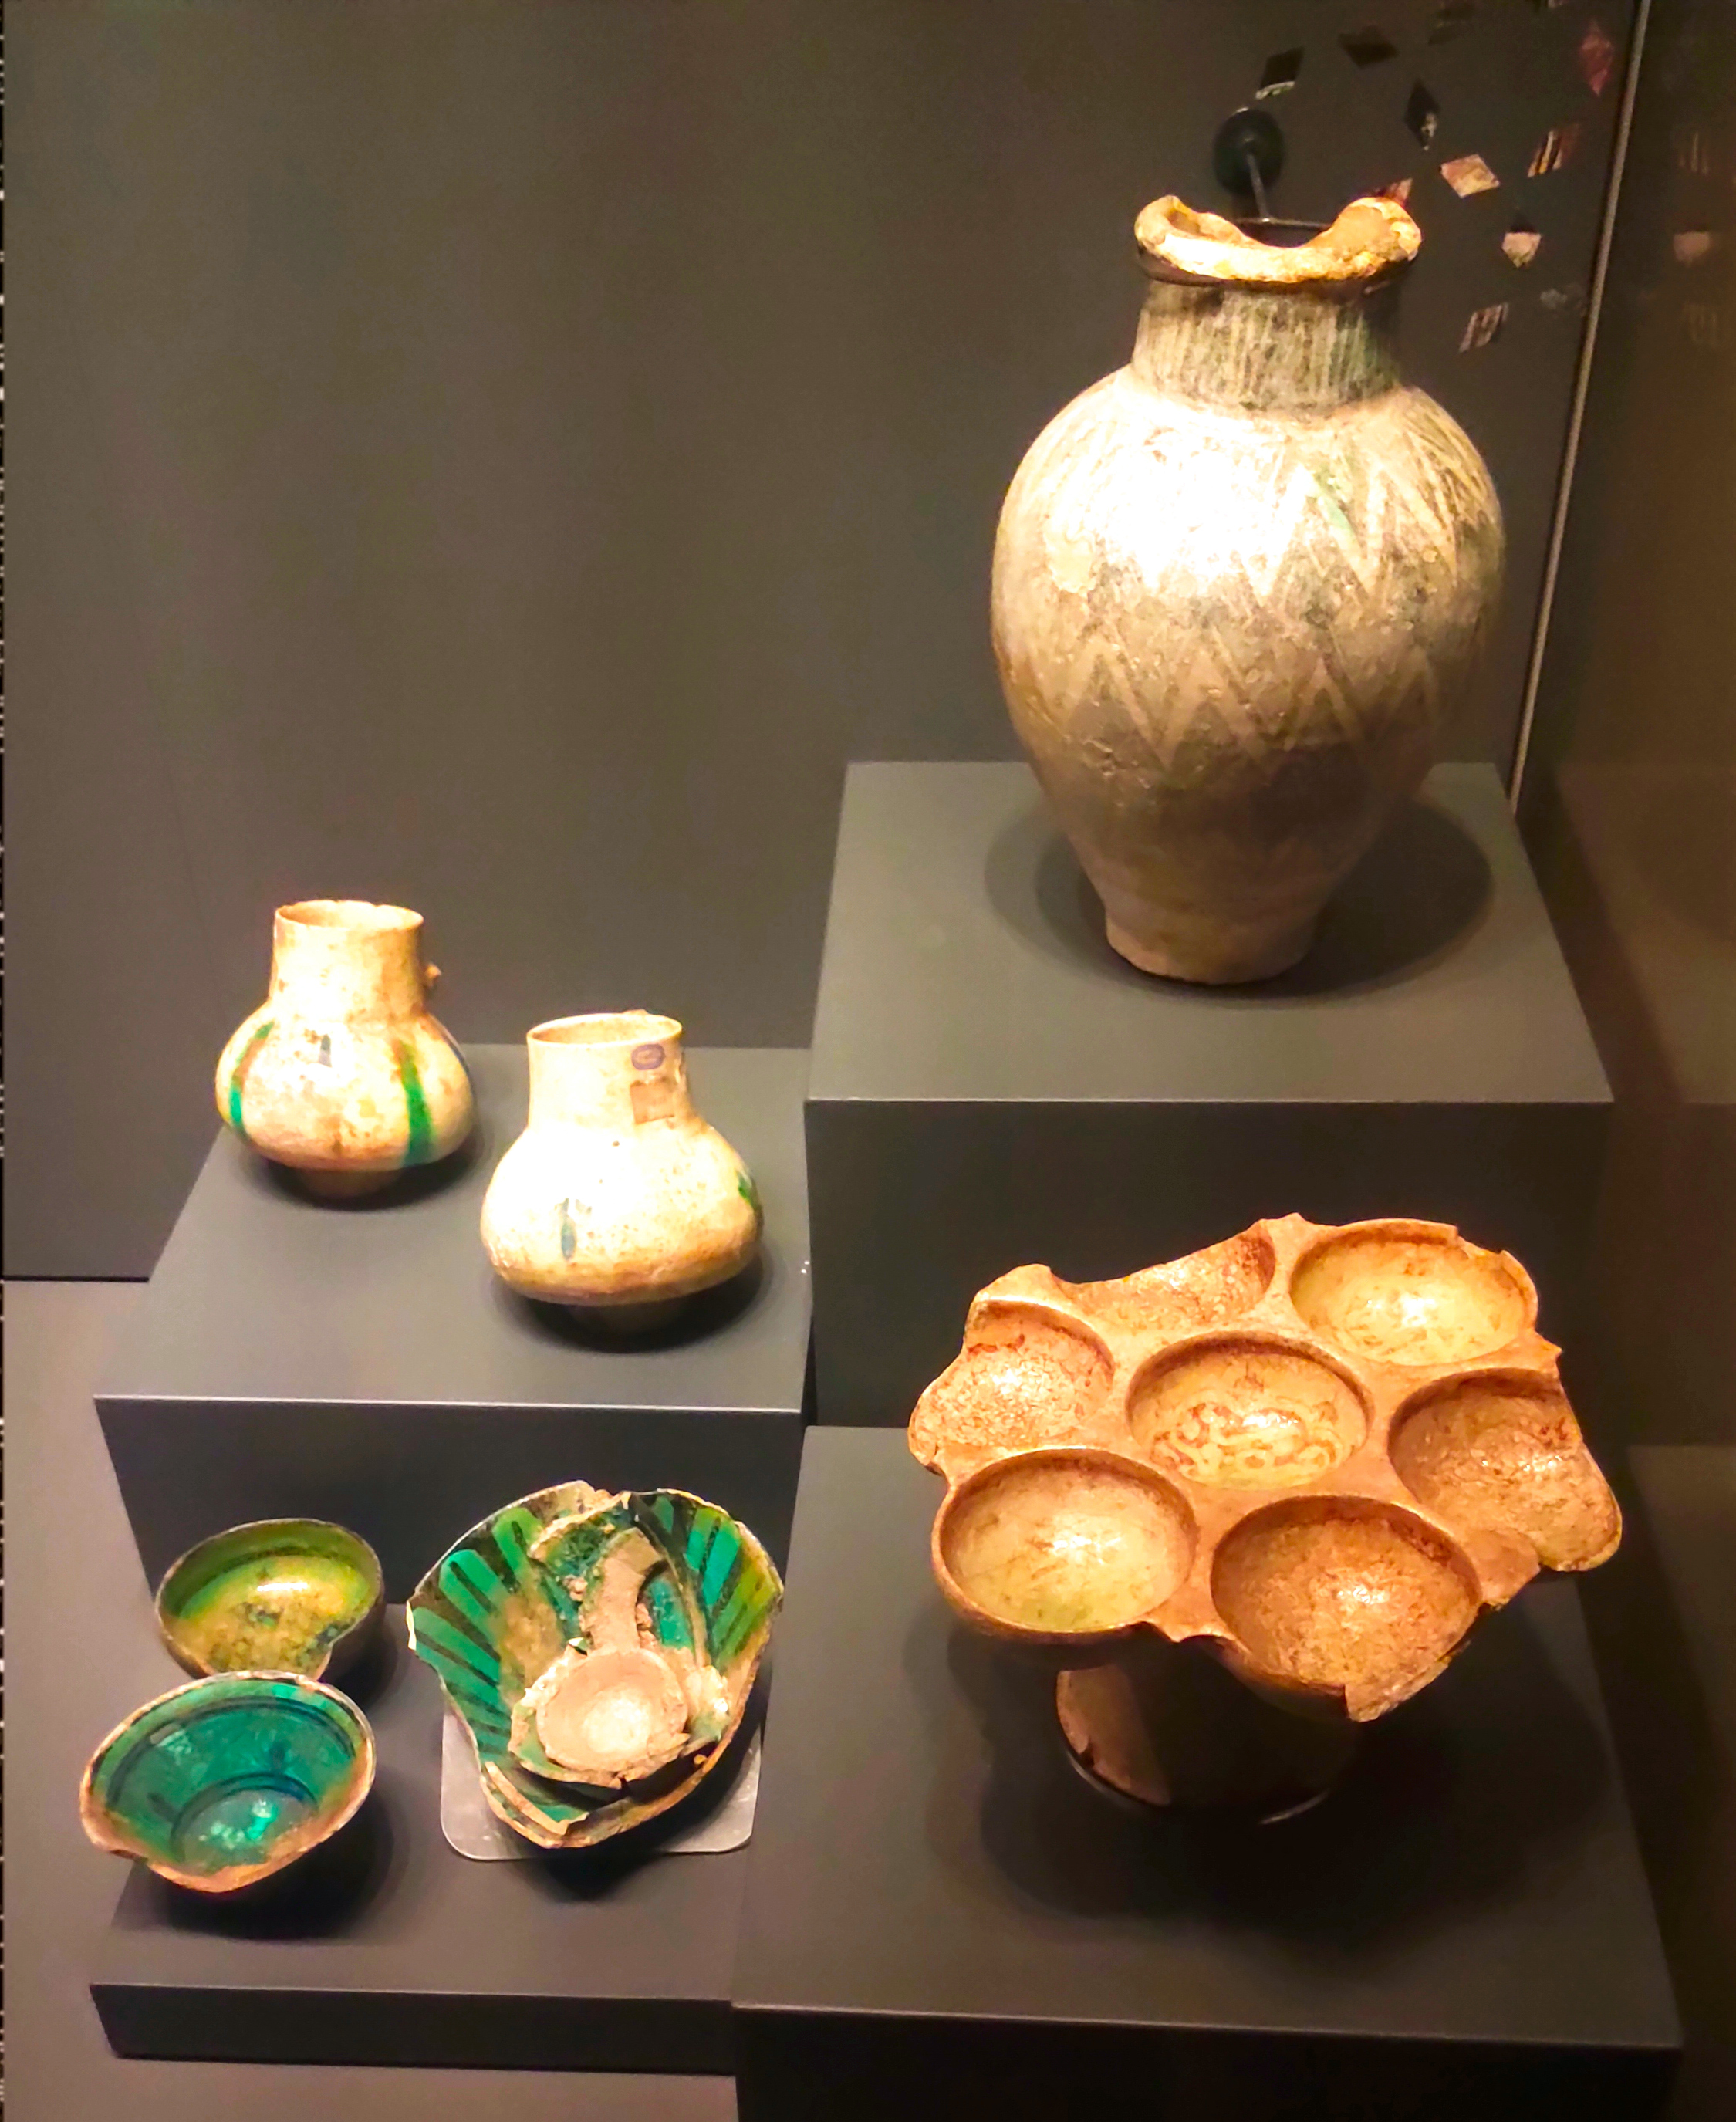
\includegraphics[height=0.25\textheight, width=0.3\linewidth]{assets/seljuks_1.jpg}
        \label{fig:seljuks_1}
    }
    \hfill
    \subfigure[Selçuklu Dönemi Seramikleri]{
        \includegraphics[height=0.25\textheight, width=0.3\linewidth]{assets/seljuks_2.jpg}
        \label{fig:seljuks_2}
    }
    \hfill
    \subfigure[Selçuklu Dönemi Seramikleri]{
        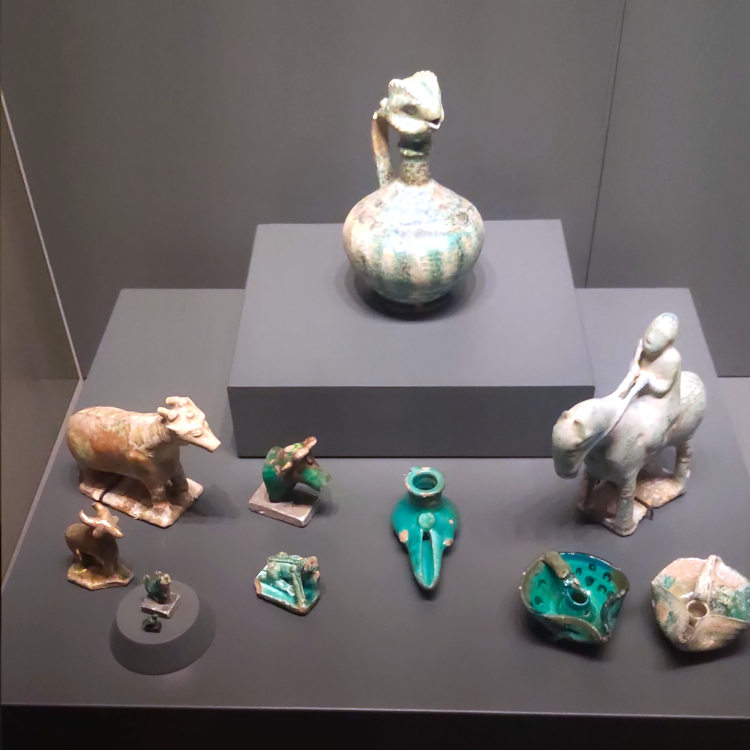
\includegraphics[height=0.25\textheight, width=0.3\linewidth]{assets/seljuks_4.jpg}
        \label{fig:seljuks_4}
    }
    \vspace{10pt}
    \subfigure[Selçuklu Seramik Yıldızı]{
        \includegraphics[height=0.25\textheight, width=0.3\linewidth]{assets/seljuks_3.jpg}
        \label{fig:seljuks_3}
    }
    \hfill
    \subfigure[Kaçar Dönemi Kalmlikler]{
        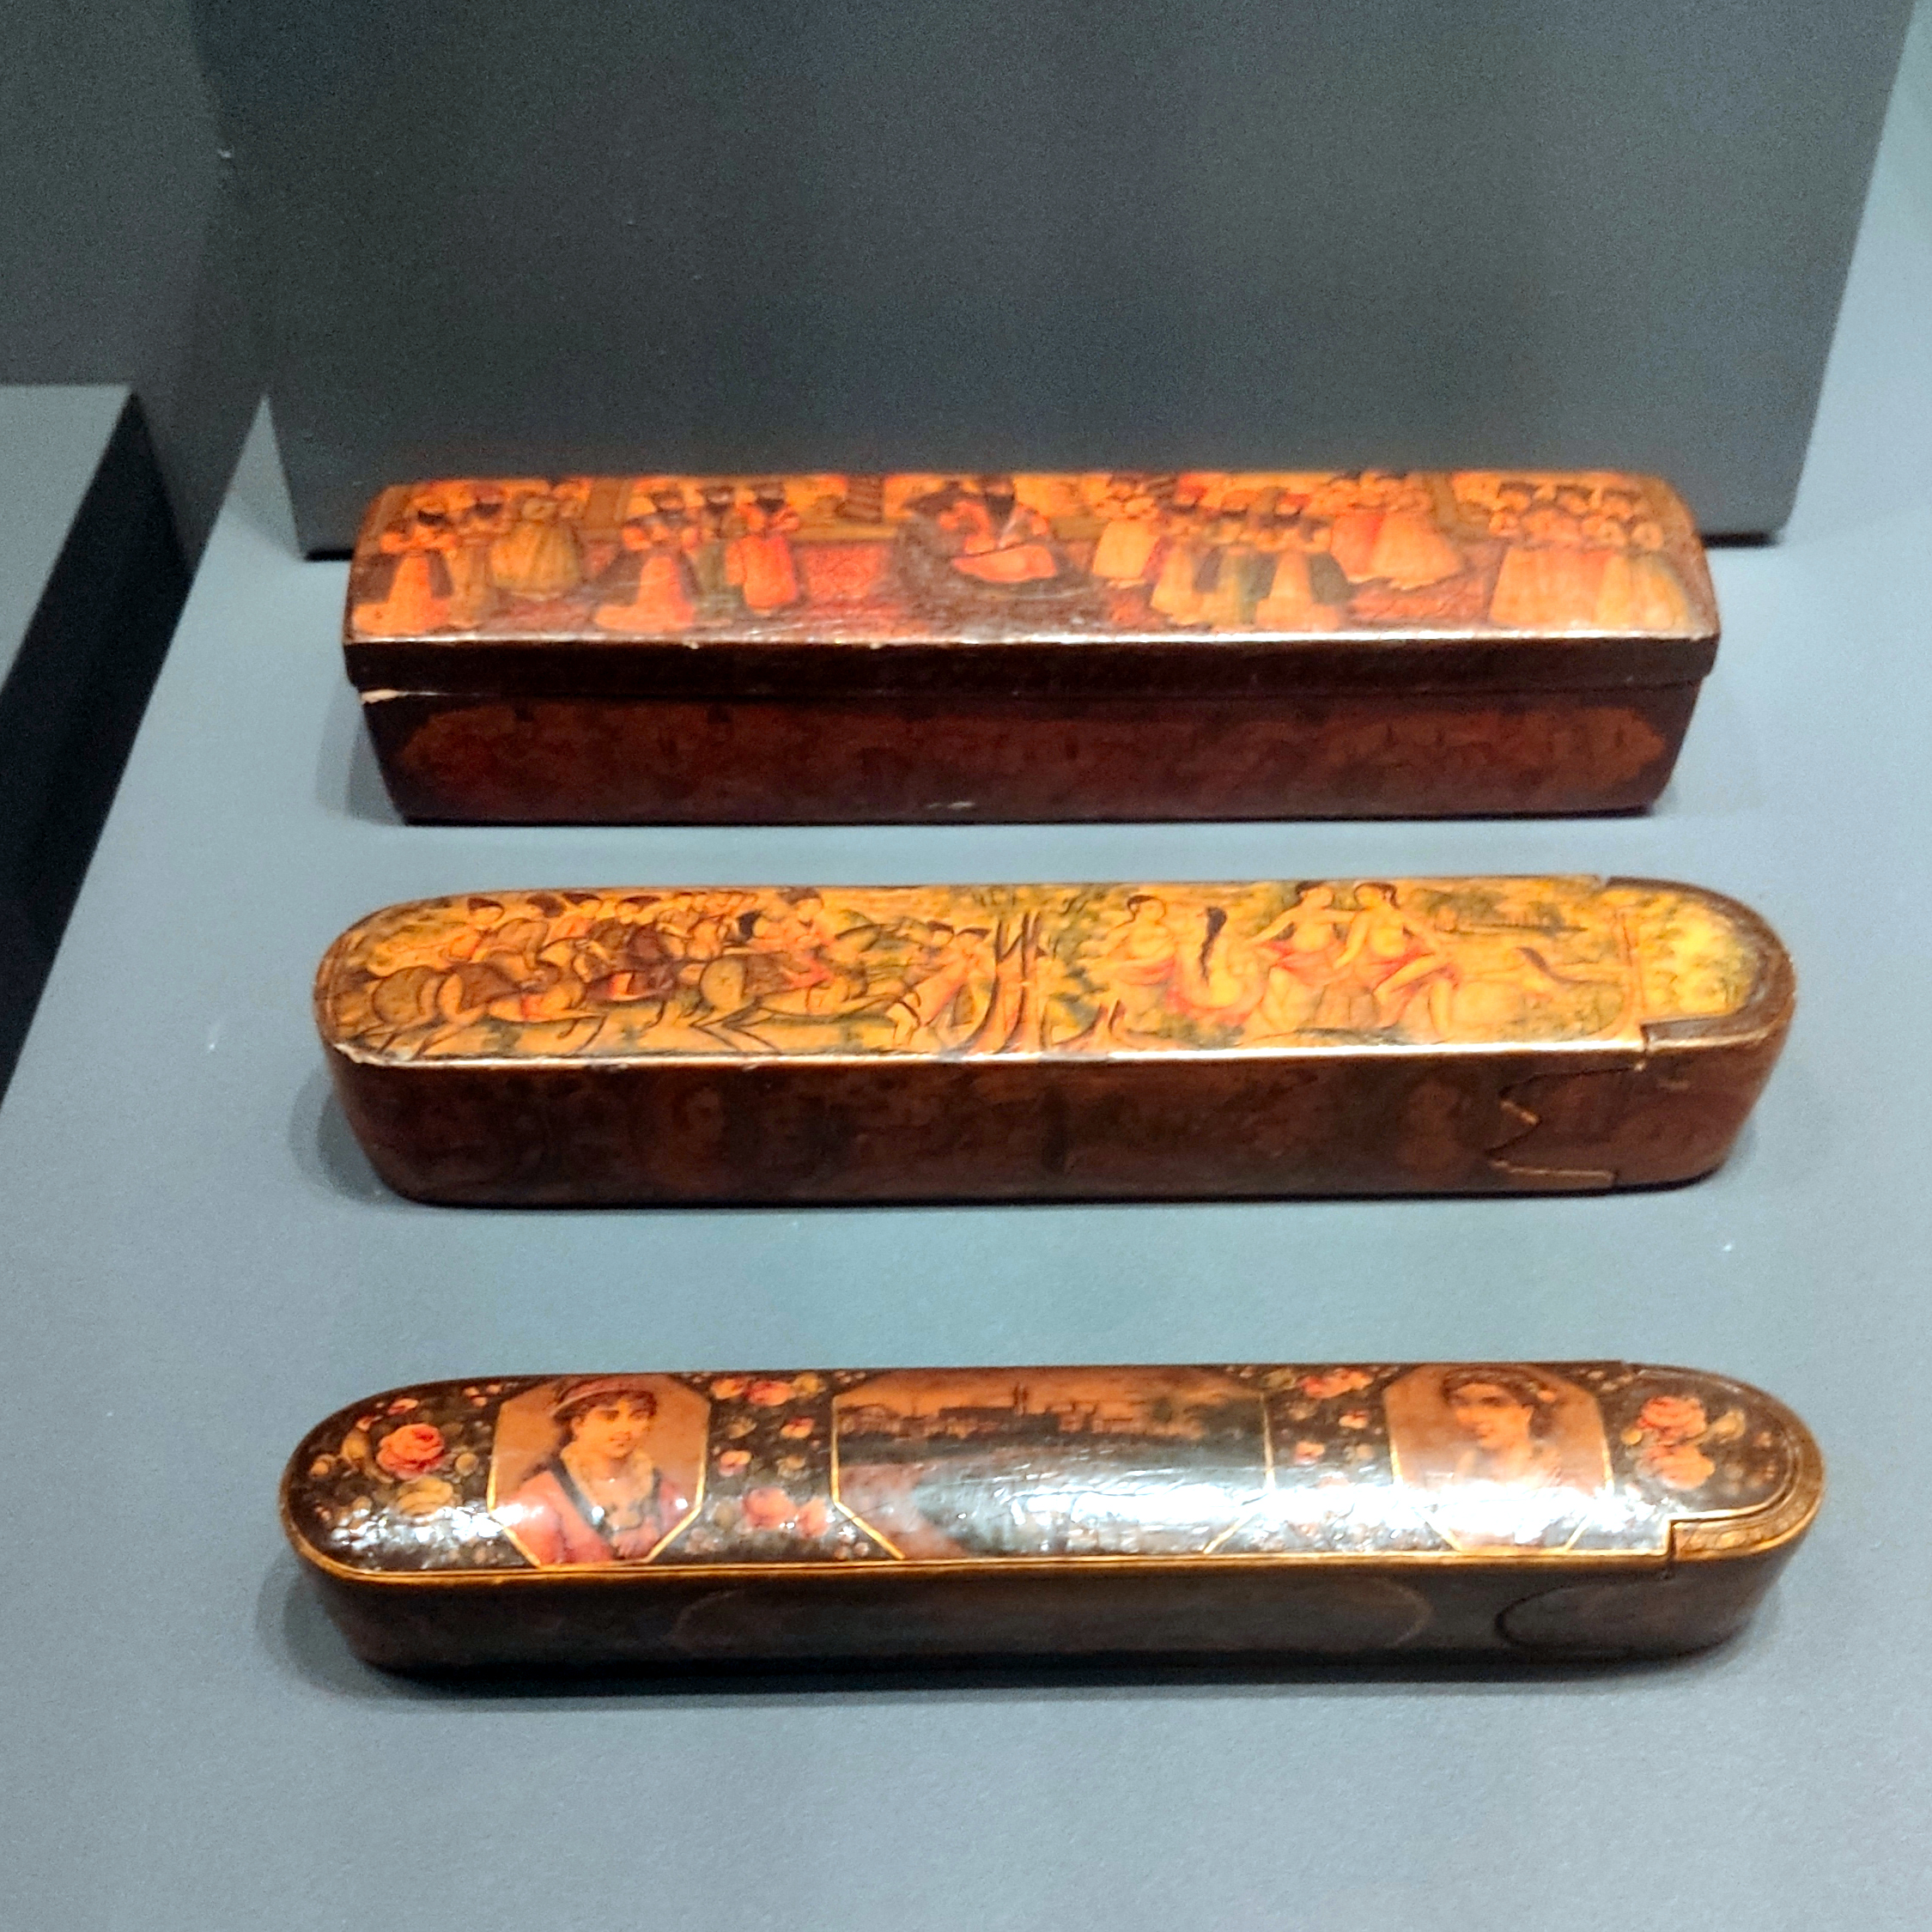
\includegraphics[height=0.25\textheight, width=0.3\linewidth]{assets/qajars_1.jpg}
        \label{fig:qajar_1}
    }
    \hfill
    \subfigure[Kaçar Dönemi Lake Oyun Kartları]{
        \includegraphics[height=0.25\textheight, width=0.3\linewidth]{assets/qajars_2.jpg}
        \label{fig:qajar_2}
    }
    \caption{Diğer Eserler}
    \label{fig:other_pieces}
\end{figure}